\chapter{Implementation}

\section{Structure}

\subsection{Overview}

Based on the project algorithm design, its Java implementation unit complies with the specified structure and thus maintain the two core phases ($Analyse$ and $Generate$). However, hard code requires extra handling of data input and output. Hence additional two phases are added: $Scan$ and $Monitor$, which read and display input respectively. Moreover, the differences in data type of different iterations require extra treatment would be too clunky to append to the $Analyse$ phase. Thus, another phase is in line: $Sub-Analyse$, which inherits $Analyse$ range-analysing functions while having additional threshold check (for density) and handle elimination round for partly-covered tuples.  

The implementation process can now be divided into five Phases instead of two from the original algorithm. The reasoning is assessed in details below:

\begin{table}[!htbp]
\caption{5-Phase Implementation and Reasoning}
\label{table:table4_6}
\centering
\begin{tabular}{lc}
	\toprule
	\textbf{Reason} & \textbf{Outcome} \\
	\midrule
	To read and pre-process data input before
analysis & Phase I Scan \\
	To comply with the original structure	& Phase II Analyse \\
	To comply with the original structure	& Phase II Generate \\
	To adapt to different iteration needs	during
data analysing process & Phase IV Sub-Analyse \\
	To monitor and record the result & Phase V Monitor \\
	\bottomrule
\end{tabular} 
\end{table}


From Table 4.1, a detailed structure for the programme can be presented visually in an Activity Diagram below:

\begin{figure}[!htbp]
    \centering
    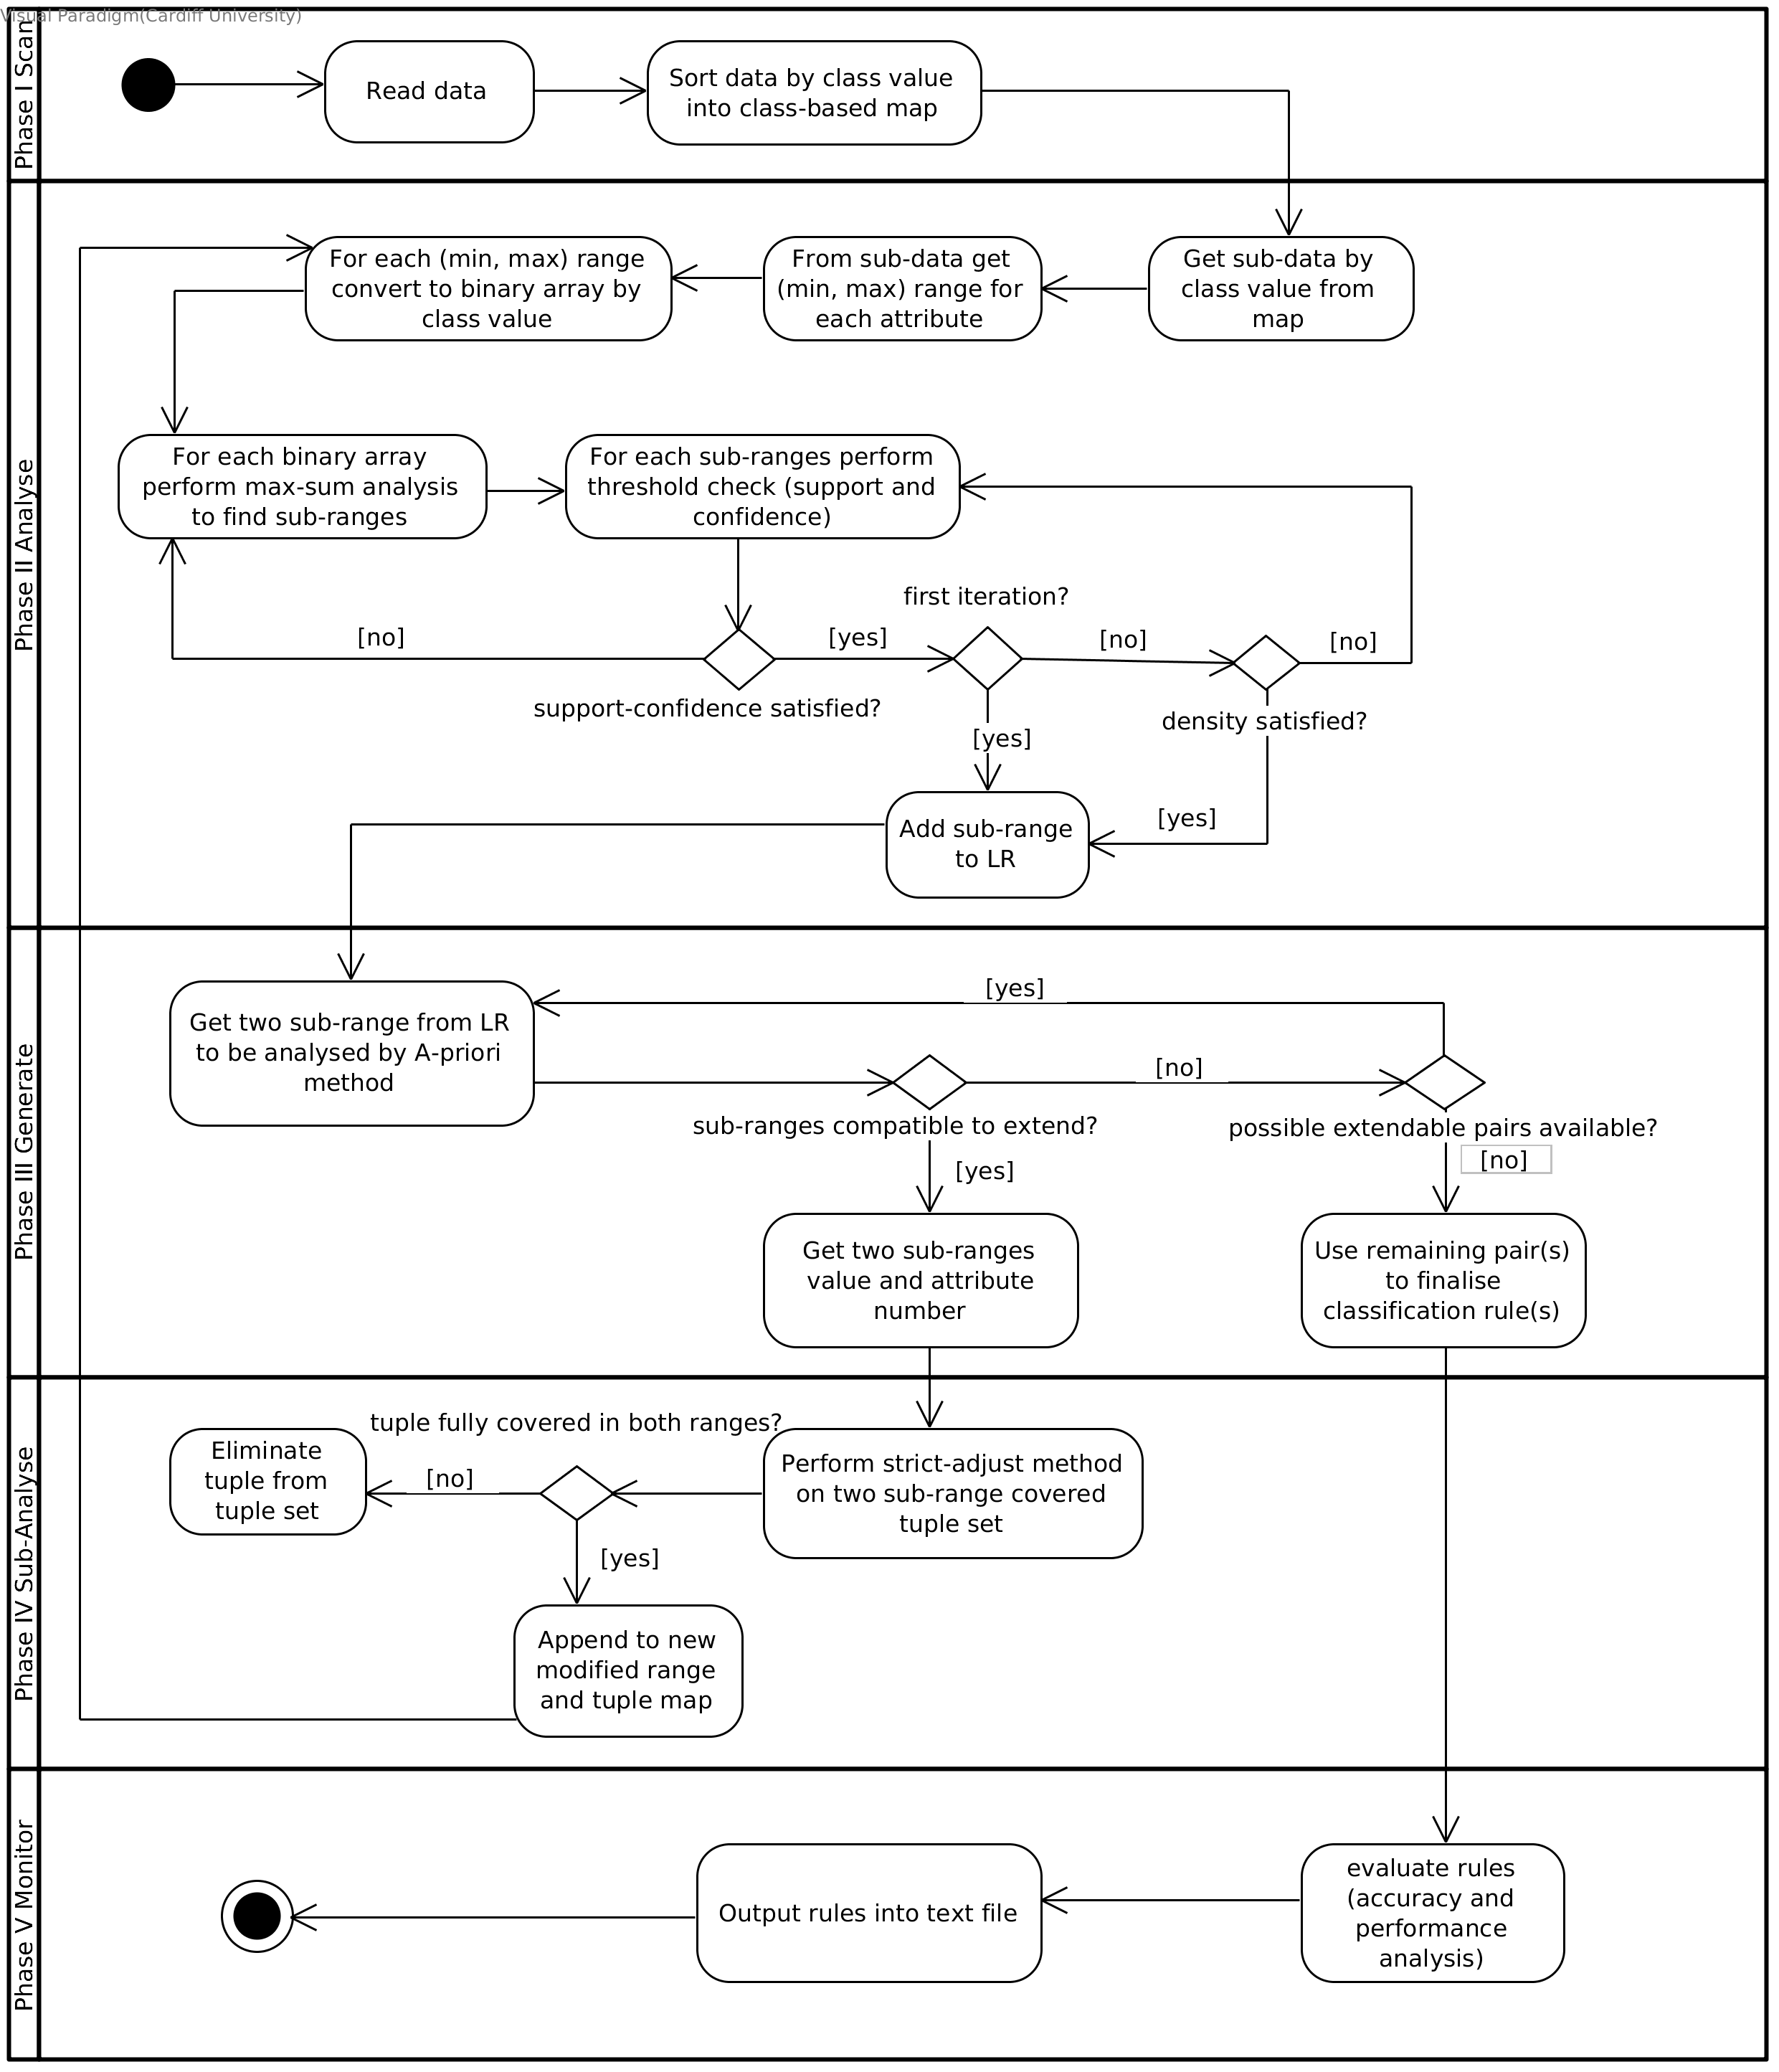
\includegraphics[width=6.5in]{figures/activity_overview}
    \caption[Class overview: Activity Diagram]{Class overview: Activity Diagram}
    \label{fig:figure4_1}
\end{figure}


Details will be discussed in sections below for each phase. To demonstrate the structure visually, a Class Diagram and an Activity Diagram is shown for each phase, that is represented by each class. Reason is because Class Diagram is the most common representation for an overview within and between classes [SRC]. A Sequence Diagram could have been an alternative to Activity Diagram; however, Sequence Diagram fails to demonstrate the actual data flow as the programme needs to call different functions or initialise different objects in different iteration. It means the sequences between classes change depending on which round the programme is on, thus not shown accurately in one data flow chart as in Sequence Diagram [SRC]. Therefore, to demonstrate the purpose of classes, Activity Diagram is in use.

\subsection{Phase I Scan}

\begin{description}

\item[Aim: ] There are three aims within this phase or class:
\begin{itemize}
	\item{To read data from \texttt{.csv} file} 
	\item{To sort data into sub-data pools using class values found when reading data in} 
	\item{To pass these data into the next phase or class ($Analyser$} 
\end{itemize}

\item[Input: ] This class input is the data itself:
\begin{itemize}
	\item{Pre-processed .csv file (no null values within attributes and the order of element in an instance is {attribute $1$, attribute $2$,..., attribute $N$, class $C$}}
\end{itemize} 

\textit{Reason: } Initial plan included an extra processing unit for filtering csv file when value is Null. However, time constraint did not allow the construction of this unit. Hence the programme only consider pre-processed csv data at the time the report is written.

\item[Output: ] This class output are data taken from input source:
\begin{itemize}
	\item{\texttt{AllTuples}: A list of all instances of the data - a list of tuples that are presented as lists.}
	\item{\texttt{AllClassMap}: A partitioned map that contains class values as keys that are connected to their relevant sub-data (list of instances) as values.}
\end{itemize}
  
\textit{Reason: } Data taken from input sources need separate containers for different purpose: \texttt{AllTuples} is required to provide access to all original data. On a different note, \texttt{AllClassMap} is required to get the class-based data partition since the key efficiency of this algorithm is to `divide and conquer' on data partitions guided by class tag [SRC]

\item[Data type: ] \texttt{LinkedList} (for tuples), \texttt{LinkedHashMap} (for class-based data partitioned map)

\textit{Reason: } A \texttt{List} - without specified inner data type - is used for tuples since it needs multiple types of data (e.g. float number, string class value, integer ordered number). In this case, \texttt{LinkedList} is used instead of \texttt{ArrayList} for two reasons: Firsrly, its ability to add and remove first and last elements more quickly than the alternative [SRC]. It is necessary to retrieve class value in each tuple at faster rate as class value is the last element in the tuple. Secondly, \texttt{LinkedList} or any type of \texttt{Linked}-collection type means its  A set of tuples thus casts as \texttt{LinkedList<LinkedList>}.

Similarly, a \texttt{LinkedHashMap} is used for faster retrieval rate an. A \texttt{HashMap} is used for storing partitioned sub-data from class values since each partition of data needs to be recorded with its unique class value. It has String class as key and \texttt{LinkedList<LinkedList>} List of all tuples as values. 

\item[Class diagram: ] 

Its class diagram is in Figure 4.1, showing two features/methods:
\begin{itemize}
	\item{scanData()} \\
	This method initialises two scanners, one to scan line-by-line data from csv file (i.e. tuples) and one to scan in-line elements (i.e. attributes).
	It processes data into 1) allTuple (where all instances are recorded from the first scanner) and 2) Class values, Tuple order numbering and Tuple attributes (which is sorted by the second scanners).
	The Class values become the parameter for the next method, where it helps create the Map that connects Class value to relevant set of Tuples.
	\item{sortData()} \\
	This method groups sets of tuples according to their Class value by checking their last String element. It sorts and partitions allTuple into sub-data pools, which are then passed on as parameter to the new class ($Analyser$).
	
\end{itemize}

\begin{figure}[!htbp]
    \centering
    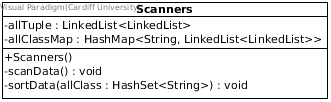
\includegraphics[width=4in]{figures/class_scanners}
    \caption[A Class Diagram for Phase I Scanners]{A Class Diagram for Phase I Scanners}
    \label{fig:figure4_2}
\end{figure}

\item[Activity diagram: ] 

FIG PLS

\end{description}

\subsection{Phase II Analyse}

\begin{description}

\item[Aim: ] Being the core module of the programme, there are important aims for this phase or class:
\begin{itemize}
	\item{To find (min, max) range for each attribute from class-based map.} 
	\item{To convert (min, max) range to binary array, which is ready for max-sum analysis.} 
	\item{To perform max-sum analysis on (min, max), aim to obtain at least one sub-optimal range, which is ready for the threshold test.} 
	\item{To perform threshold check. As discussed, this check diverses depending on which iteration. However, support and confidence is always required thus appear in this phase or class.} 
	\item{To modify the new sub-data pools for the next iteration. Since data set would shrink after pruning process from max-sum and (if applicable) strict-adjust method, current data set is frequently changing. Threshold measures, however, are calculated depending on these sets, thus makes this modification step necessary.} 
	\item{To pass the modified sub-data pools as well as new sub-ranges to the next phase or class ($Generator$).} 
\end{itemize}


\item[Input: ] This class input is the original dataset and the class-based data map from passed on from previous class:
\begin{itemize}
	\item{\texttt{allTuple}:  all original instances in dataset.} 
	\item{\texttt{allClassMap}: with key as class tag and value as relevant sub-data partition.}
\end{itemize}

\textit{Reason: } \texttt{allClassMap} is needed for the class-guided search for the rest of the programme. This map, however, changes as the sub-data pool changes throughout the cycle. Therefore, \texttt{allTuple} is needed to refer back to the original, pre-modification input when necessary.

\item[Output: ] A list of sub-ranges in float values that passed the support-confidence check (\texttt{attributeRangeList}). It also returns a modified version of allClassMap, which \texttt{AllClassMap} is now divided into two maps: \textit{attributeRange} and \textit{attributeTuple}.
  
\textit{Reason: } As required for the next $Generate$ phase, \texttt{attributeRangeList} stores potential associated ranges for new combination. 
Map, however, diversifies into two: 
\begin{itemize}
	\item One for storing sub-ranges (that are also stored in \texttt{attributeRangeList})for each attributes. That means \texttt{attributeRangeMap} has its key quantity equal to the number of attributes, and each key maps to at least one sub-range found from analysing methods.
	
	\item One for storing tuples that each sub-range in \texttt{attributeRangeMap} covers. That means \texttt{attributeRangeMap} has its key quantity equal to the number of sub-ranges available (that are also recorded in \texttt{attributeRangeList}), and each key maps to a list of tuples that is covered by that range.
	
Initially, only \texttt{attributeRangeMap} was implemented as it was thought that only attribute and its sub-ranges were necessary to be recorded formally. Tuples covered by sub-ranges were thought to be retrievable by tracing back to the original \texttt{AllClassMap}.
	
However, as data was partitioned further the longer the algorithm persisted, there was no fixed map that remained relevant for the entire duration of the programme. With the dynamic nature of tuple sets, it was safer to recorded them right when their sub-ranges were being processed. Thus there was a need for the additional \texttt{attributeTupleMap}.
\end{itemize}

\item[Data type: ] For \texttt{attributeRangeMap}, a \texttt{LinkedHashMap} with \texttt{LinkedList<Integer>} as keys and \texttt{LinkedList<LinkedList<Float[]>>} as values is used. This map stores attribute number as key (thus \texttt{Integer} type cast) and ranges as value (thus \texttt{LinkedList<Float>} type cast). It must be noted that despite attribute number being a singular integer (from $1$ to $n$), \texttt{LinkedList} is implemented since attributes' ranges are combined at Generate phase. That means attribute number must be expandable to manage this new combination (e.g attribute $1$ and $2$ has associated ranges of $[1.1,1.5]$ and $[2.2, 2.6]$. Once these two ranges are combined to form larger ranges, attribute numbers are also combined i.e. to ${1,2}$ to manage this combined range in the map) - hence need for a \texttt{List}. Likewise, \texttt{LinkedList<Float>} is sufficient to manage a single range; when there are multiple ranges to be stored, an outer \texttt{LinkedList} must be used.

Similarly, For \texttt{attributeTupleMap}, a \texttt{LinkedHashMap} with \texttt{LinkedList<LinkedList<Float[]>>} as keys and \texttt{LinkedList<LinkedList>} as values. Keys in \texttt{attributeTupleMap} are \texttt{attributeRangeMap} values; the cross-reference makes for a convenient key retrieval between two maps. 

\item[Class diagram: ] 

Its class diagram is in Figure 4.3, which additionally shows a parentage link to $SubAnalyser$ class for Phase IV $Sub-Analyse$. It is the only instance of inheritence in the programme: $Analyser$ is used in the first iteration and its framework is re-used for code efficiency in $Sub-Analyser$ for second iteration onwards. For this subsection, only $Analyser$ is discussed; $SubAnalyser$ is to be explained in the next subsection.

Class $Analyser$ contains seven features/methods:

\begin{itemize}
	\item{maxMin()} \\
	This method is responsible for collecting (min, max) ranges for each attribute. For each of the Class value in the map, it goes through each attribute value of every corresponding tuples. A \texttt{Collections.sort()} method is applied to find the minimum and maximum value of each attribute. In the first iteration, only one range is found for each attribute.
	
	For each range, it then appends {attribute number, range} to \texttt{attributeRangeMap}. It also retrieves tuples that are covered under this range and appends {range, range-covered tuple} to \texttt{attributeTupleMap}. 
	
	These two maps, accompanied by the Class value, are passed onto the next method, \texttt{convertToBinary} to prepare binary array for max-sum analysis.
	
	\item{convertToBinary()} \\
	For each attribute in \texttt{attributeRangeMap}, this method retrieves the respective (min, max) range. Each range is used as key to search in \texttt{attributeTupleMap} to obtain tuples that are covered by this range. It then goes through each tuple to retrieve its Class tag and if this tag matches the Class value received from previous method, it appends $1$ to a new \texttt{binaryList}, otherwise appends $-1$. 
	
	This binary list is sent to the next method \texttt{maxSum()} for sub-range analysis.
	
	\item{maxSum()} \\
	For each of the binary list, this method performs a similar analysis to Kadane's max-sum algorithm [SRC]: Starting with a $sum$ of $0$, it traverses through the list values while adding this value to the initial $sum$, also keeping track of the element position in an $attributePosition$ array. If $sum$ is positive, it moves on while taking the same action. However, if it gets negative, it resets the $sum$ to $0$ and also restart the $position array$. This essentially means that the current array contains too many wrong class tag if continued (i.e. too many $-1$s), and thus not necessary to proceed into more negatives. 
	
	However, while a new $attributePosition$ array is created starting from this position, the current array is recorded instead of discarded, which is also considered as a sub-range ready for next iteration. This step differentiates this method from the original Kadane's since Kadane's seeks for only one optimal range, constrasting to this method where multiple sub-ranges are desired.
	
	The process is repeated until the end of array is reached. The outcome can be 1) no $attributePosition$ array or sub-ranges found, 2) one $attributePosition$ arrayor sub-range found, or 3) multiple $attributePosition$ array or sub-ranges found. Regardless, if available, sub-ranges (in $attributePosition$ array format) are recorded into an \texttt{List} and passed onto next method, \texttt{checkSupportConfidence()}, for threshold test. 
	
	It must be noted that, initially, whenever a $attributePosition$ array is found, \texttt{checkSupportConfidence()} is called straight away so a threshold test is performed whenever $sum$ turns negative. However, it means that \texttt{checkSupportConfidence()} might be called excessively in the case of a negative streak for $sum$, thus might be safer to call it after max-sum is finished. 
	
	\item{checkSupportConfidence()} \\
		
	
	\item{convertPositionToRange()} \\
	\item{appendToMap()} \\
	\item{getAttributeRangeList()} \\
\end{itemize}
	

\begin{figure}[!htbp]
    \centering
    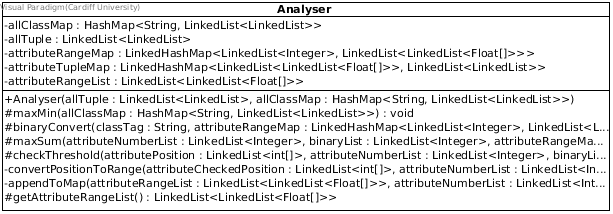
\includegraphics[width=4in]{figures/class_analyser}
    \caption[Class Diagram for Phase II Analyse]{Class Diagram for Phase II Analyse}
    \label{fig:figure4_3}
\end{figure}

\item[Activity diagram: ] 

FIG PLS
\end{description}


FOR FORMATTING

\subsection{Phase III Generate}

\subsection{Phase IV Sub-Analyse}

\subsection{Phase V Monitor}

\section{Development Process}

\subsection{Planning}
\subsection{Technical Platforms}
\subsection{Version Control}





